\section{Durchführung und Aufbau}
\label{sec:Durchführung}

\subsection{Laser}
\label{sec:AufbLaser}
Für dieses Experiment wird ein Infrarot Diodenlaser als Quelle für kohärentes Licht verwendet. Verwendet wird ein sgn. Littrow-Aufbau, welcher es ermöglicht ein eingebautes Beugungsgitter
zu verstellen. Zusätzlich zum Gitter hat der Laser bereits einen Kollimator verbaut, welcher für einen parallelen Strahlengang sorgt.
Außerdem werden eine Infrarot-sensitive Kamera, ein Bildschirm um das Bild auszugeben benötigt. Für die Justierarbeiten erweist sich eine Detektorkarte als praktisch, welche es 
ermöglicht das Licht mit dem bloßen Auge zu sehen. Außerdem ist darauf zu achten, dass die Temperatur des Lasers konstant auf 50\,°\unit{\celsius} gehalten wird damit die für das Rubidium geeignete Wellenlänge erzeugt wird.

%This experiment uses a diode laser as a source of coherent light. The light can be adjusted by a turning a screw that changes the angle of a diffraction grating. 
%In addition to that, a so called collimator is used to narrow the emitted light to a smaller, more precise beam. 

\subsection{Lasergranulation}
\label{sec:AufbLasergran}
Der erste Teil des Versuches besteht darin den Schwellenstrom des Lasers zu messen ab welchem es zur sgn. Lasergranulation kommt.
Der dazu verwendete Aufbau ist in \autoref{fig:Setup1} schematisch dargestellt.
\begin{wrapfigure}{r}{0.32\textwidth}
    \begin{center}
        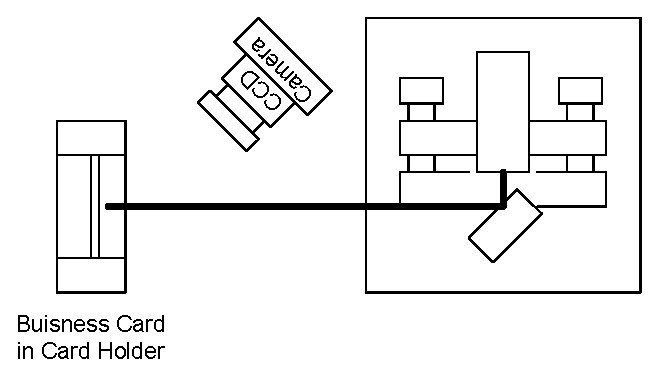
\includegraphics[width=0.4\textwidth]{Setup1.pdf}
        \caption{Aufbau zur Bestimmung des Schwellenstroms \cite{ap60}.}
        \label{fig:Setup1}
    \end{center} 
\end{wrapfigure}
Lasergranulation tritt auf, wenn kohärentes Licht auf eine Oberfläche trifft, dessen Unebenheiten in etwa die Größe der Wellenlänge haben (gleiche Größenordnung).
Nach dem Huygen'schen Prizip kann jeder Punkt einer Wellenfront als Kugelwelle verstanden werden. Aufgrund der unebenen Oberfläche kommt es dazu dass die überlagerten Kugelwellen
nicht mehr die ursprüngliche Wellenfront ausbilden sondern es zu neuen Überlagerungen kommt, die in Form eines unregelmäßigen Interferenzmusters sichtbar werden.
Erst wenn der Strom der am Laser anliegt groß genug ist, ist das abgestrahlte Licht kohärent. Vorher ist die Funktionsweise wie die eines herkömmmlichen LED's und es würde wegen fehlender 
Kohärenz zu keinerlei Streuphänomenen kommen.
Der Strom wird langsam erhöht bis die Lasergranulation auftritt.
Die Kamera wird verwendet um je ein Bild unter- und überhalb des Schwellenstroms zu machen.


\subsection{Rubidium Floureszenz und dessen Spektrum}
\label{sec:Rubi}
%For the study of Rubidium's Flourescence, the experiment used for the first part of this experiment needs to be modified.
%The Rubidium Cell, which is placed between Field Coils and inside a heater to control its temperature, is set up between the ND Filter Holder and the laser.
Um die Floureszenz von Rubidium zu untersuchen wird eine mit Rubidium gefüllte Zelle in den Strahl platziert. Diese Zelle wird zwischen Feldspulen und in einem Heizer platziert um die Temperatur konstant zuhalten.
Im Anschluss muss der Strahl so eingestellt werde, dass die Floureszenz als heller leuchtender Strich deutlich in der Kamera zu sehen ist. Der Strom wird weit über den Schwellenstrom gedreht, um sicherzugehen dass die Leuchtkraft des Lasers
ausreichend ist. Um nun die für Rubidium passende Frequenz zu erreichen, kann der Piezo-Kristall im Laser über eine Veränderung des an ihm anliegenden Strom so verformt werden, dass dieser 
den Winkel des Gitter und die Resonanz des inneren Resonators verändert.
Der verwendete Aufbau ist in \autoref{fig:Setup2} dargestellt.
\begin{figure}
    \centering
        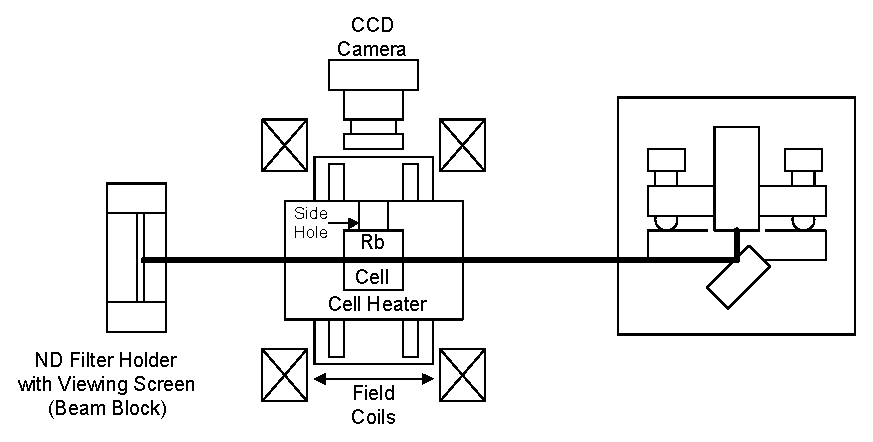
\includegraphics[width=0.8\textwidth]{Setup2.pdf}
        \caption{Aufbau zur Messung der Rubidium Floureszenz \cite{ap60}.}
        \label{fig:Setup2} 
\end{figure}
Das Spektrum von Rubidium wird mit einem ähnlichen Aufbau aufgezeichnet. Hierzu muss jedoch zwischen Laser und Rubidium-Zelle ein Strahlteiler eingebaut werden, welcher den einen Teil direkt in ein Photoelement leitet
und einen anderen Teil durch die Rubidium-Zelle in einen zweiten Photodetektor leitet.
Es sind zwei Photozellen nötig, damit die auftretende Hintergrundstrahlung herausgefiltert werden kann. So kann das Signal das ersten Detektors später vom zweiten abgezogen werden um ein klareres Bild zu erzeugen.
Es ist zu beachteten, dass alle vier typischen Abfälle im Spektrum durch ein und dieselbe Mode dargestellt werden, da es sonst zu Sprüngen kommen kann, welche dafür sorgen, dass die Intensität plötzlich abfällt.